%% -*- coding: utf-8; -*-

\documentclass[
  master
  brazilian
]{ThesisPUC}


%%%
%%% Additional Packages
%%%

% \usepackage[brazilian]{babel}      %% in ThesisPUC.cls
% \usepackage[utf8]{inputenc}        %% .
% \usepackage[T1]{fontenc}           %% .
% \usepackage{lmodern}               %% .
% \usepackage[pdftex]{graphicx}	%% .

  \usepackage{tabularx}
  \usepackage{multirow}
  \usepackage{multicol}
  \usepackage{colortbl}
  \usepackage[%
    dvipsnames,
    svgnames,
    x11names,
    fixpdftex
  ]{xcolor}
  \usepackage{numprint}
  \usepackage{textcomp}
  \usepackage{booktabs}
  \usepackage{amsmath}
  \usepackage{enumitem}
  \usepackage{amssymb}
  \usepackage{textcomp}
% \usepackage{etoolbox}

%% numprint 
\npthousandsep{.}
\npdecimalsign{,}

%% ThesisPUC option
%% \tablesmode{figtab} %% [nada, fig, tab ou figtab]


%%%
%%% Counters
%%%

%% uncomment and change for other depth values
%% \setcounter{tocdepth}{3}
%% \setcounter{lofdepth}{3}
%% \setcounter{lotdepth}{3}
%% \setcounter{secnumdepth}{3}


%%%
%%% New commands and other global definitions
%%%

% -*- coding: iso-8859-1; -*-

\newcommand{\degree}{\ensuremath{^\circ}}

\newcommand{\cetem}{Centro de Tecnologia Mineral}

%\newcommand{\cetem@ini}{CETEM}
%\newcommand{\ini}[1]{\renewcommand{\cetem@ini}{#1}}
\newcommand{\CETEM}{CETEM}


%%%
%%%
%%%
\newcommand{\mybulletOB}{%
  % \textbullet
  % \checkmark
  $\triangleright$
  %\textopenbullet
}

\newcolumntype{L}{>{\raggedright \arraybackslash}X}
\newcolumntype{R}{>{\raggedleft \arraybackslash}X}
\newcolumntype{C}{>{\centering \arraybackslash}X}
\newcolumntype{M}[1]{>{\centering\hspace{0pt}}m{#1}}

\newcommand{\mrcel}[2]{%
\begin{tabular}[c]{@{}c@{}}#1\\#2\end{tabular}}

\newcommand{\mrcell}[2]{%
\begin{tabular}[l]{@{}l@{}}#1\\#2\end{tabular}}

\newcommand{\mrcelthree}[3]{%
\begin{tabular}[c]{@{}c@{}c@{}}#1\\#2\\#3\end{tabular}}

\newcommand{\mrcelcolorg}[2]{%
\begin{tabular}{l}\rowcolor{Gainsboro}#1\\#2\end{tabular}}

\newcommand{\tbthreeblabla}[3]{%
\begin{tabular}{ l @{\extracolsep{2mm}}X }
  \mybulletOB #1
  \mybulletOB #2
  \mybulletOB #3
\end{tabular}}

\newcommand{\mytbcimg}[3]{%
  \multicolumn{1}{C}{\parbox[c]{#1}{\includegraphics[width=#2]{#3}}}}

%%%
%%% In table-2.1
%%%

\newcommand{\colmund}[1]{\npmakebox[abcdef][c]{#1\degree}}


%%%
%%% Misc.
%%%

\usecolour{true}


%%%
%%% Titulos
%%%

\author{José Flávio Cavalcante Barros Júnior}

\advisor{Edward Hermann Haeusler}{Prof.}

\title{Compressão de Provas: uma análise sobre técnicas e uma proposta de estrutura para representar provas}

% \titleuk{Development of a digital microscopy system for automatic classification of hematite types in iron ore}

%% \subtitulo{Aqui vai o subtitulo caso precise}

\day{04}
\month{Março}
\year{2019}

\city{Rio de Janeiro}
% \CDD{620.11}
\department{Informática }
\program{Informática }
\centro{Centro Técnico Científico }
\university{Pontifícia Universidade Católica do Rio de Janeiro}
\uni{PUC-Rio}


%%%
%%% Jury
%%%

\jury{%
%   \jurymember{}{Prof.}
%     {Universidade Federal de Minas Gerais}{UFMG}
%   \schoolhead{}{Prof.}
}


%%%
%%% Resume
%%%

\resume{%
  
  }


%%%
%%% Acknowledgment
%%%

\acknowledgment{%
  \noindent %I would like to first thank my advisor ...
  \bigskip

  \noindent %Then I wish to thank ...
}


%%%
%%% Catalog prekeywords
%%%

\catalogprekeywords{
  
}


%%%
%%% Keywords
%%%

\keywords{%
%   \key{Minério de Ferro;}
%   \key{Cristais de Hematita;}
%   \key{Microscopia Digital;}
%   \key{Análise de Imagens;}
%   \key{Classificação;}
%   \key{Microscopia de Luz Polarizada.}
}

\keywordsuk{%
%   \key{Iron Ore;}%
%   \key{Hematite Crystals;}%
%   \key{Digital Microscopy;}%
%   \key{Image Analysis;}%
%   \key{Classification;}%
%   \key{Polarized Light Microscopy.}%
}


%%%
%%% Abstract
%%%

\abstract{

}

\abstractuk{

}


%%%
%%% Dedication
%%%

\dedication{
}

%%%
%%% Epigraph
%%%

\epigraph{
 
}
\epigraphauthor{}
\epigraphbook{}


%%%
%%% 
%%%

\begin{document}

  %% -*- coding: utf-8; -*-

\begin{thenotations}

  \noindent
  \begin{tabular}{ll}
    % ADI -- Análise Digital de Imagens\\
    % BIF -- \textit{Banded Iron Formation}\\
  \end{tabular}

\end{thenotations}

  % -*- coding: utf-8; -*-

\chapter{Introdução}

Provas matemáticas existem desde a Grécia antiga e têm o objetivo de corroborar a veracidade de uma afirmação, além de transmitir conhecimento entre especialistas através do tempo. As provas matemáticas utilizadas até o final do século XIX, conhecidas como provas informais, são geralmente construídas em linguagem natural e não possuem uma forma precisa, sendo estruturadas de acordo com a vontade do autor. Apesar de serem bastante utilizadas, as provas informais têm um importante problema: inexiste um método efetivo de verificação de erros. Entre o final do século XIX e o início do século XX, alguns matemáticos e lógicos abordaram diferentes maneiras para fundamentar a matemática através de um aparato teórico que permitisse uma checagem de erros. Entre as várias contribuições para a lógica matemática, surgiu o ramo da \textit{teoria da prova} juntamente com o conceito de prova formal.

Ao contrário das provas informais, as provas formais são estruturadas através de rigorosas regras de construção. Uma prova formal é a derivação de uma sentença (conclusão) a partir de outras sentenças (axiomas e hipóteses), tal derivação é uma sequência de sentenças, onde cada elemento da sequência é uma hipótese ou axioma, ou é resultado da aplicação de uma regra de inferência de um sistema dedutivo. Cada sentença de uma prova formal, também chamada de fórmula, é um elemento de uma linguagem formal, linguagens da Lógica Proposicional e da Lógica de Primeira Ordem são exemplos de linguagens formais.

Além da utilização puramente teórica na lógica matemática, provas formais podem ser utilizadas para diversas finalidades em diferentes contextos. No desenvolvimento de \textit{softwares}, provas podem ser necessárias para validar o funcionamento de porções de código. Na fabricação de \textit{hardwares}, um projeto de circuito pode ser validado através da prova de uma fórmula que o descreve. Em alguns casos, tais provas podem ser grandes, possuindo tamanhos exponenciais em relação ao tamanho da conclusão, o que aumenta significativamente a complexidade da construção e demanda uma automação.

A Prova Automática de Teoremas (\textit{Automated Theorem Proving} - ATP) é a área da Ciência da Computação que utiliza programas de computador para a geração automatizada ou semiautomatizada de provas. No entanto, um provador de teoremas ainda pode gerar provas muito grandes. O tamanho de uma prova pode prejudicar sua utilização prática, visto que a extração de alguma informação útil ao contexto pode se tornar inviável, além de que manipular grandes volumes de dados pode acarretar problemas de implementação para o provador. Esses problemas reforçam a importância do esforço para compressão das provas geradas e/ou na geração de provas já comprimidas.

Além de possíveis problemas de implementação nos provadores, o tamanho das provas possui algumas importantes implicações teóricas na área da complexidade computacional. Statman mostrou que o problema de determinar se uma fórmula é uma tautologia ($TAUT$) da Lógica Proposicional Intuicionista e do fragmento puramente implicacional da Lógica Minimal (M$\supset$) é PSPACE-Completo \cite{STATMAN197967}. M$\supset$ é capaz de simular a Lógica Proposicional Intuicionista através de uma tradução polinomial. Qualquer lógica proposicional com um sistema de dedução natural que satisfaça o princípio da subfórmula também possui seu respectivo $TAUT$ em $PSPACE$ \cite{Haeusler2014}. Um sistema de dedução natural que satisfaz o princípio da subfórmula é capaz de gerar provas onde cada ocorrência de fórmula é uma subfórmula da conclusão ou é uma subfórmula de alguma hipótese. Saber se $TAUT$ da M$\supset$ possui um certificado polinomial para qualquer tautologia, i.e, saber se qualquer tautologia possui uma prova de tamanho polinomialmente limitado em relação ao tamanho da conclusão, está relacionado com saber se $NP = PSPACE$.

Provas em dedução natural podem ser representadas em diferentes formatos. No estilo de Gentzen-Prawitz, as provas possuem o formato de uma árvore, onde as fórmulas são representadas pelos nós, e as regras e os rótulos de descarte são representados pelas arestas. No estilo de Ja{\'s}kowski-Fitch, as provas são sequências de passos numerados seguidos pela identificação da regra e sua referida justificativa. O tamanho de uma prova pode ser aferido a partir de diferentes pontos de vista. A quantidade de nós (Gentzen-Prawitz), a quantidade de linhas (Ja{\'s}kowski-Fitch) e até a quantidade de símbolos podem ser utilizados para mensurar o tamanho de uma prova. Para a complexidade computacional, o tamanho de uma prova é a quantidade de símbolos de sua representação.

É bem conhecido que provas podem ser muito grandes. Na M$\supset$, algumas fórmulas possuem provas em dedução natural com tamanhos com limite inferior exponencial \cite{haeusler2015many}. A redução do tamanho de provas pode ser realizada, principalmente, através de duas abordagens: gerar provas já comprimidas através de um cálculo de dedução natural que seja capaz de gerar provas menores que a dedução natural usual; comprimir provas em dedução natural que já tenham sido geradas.

Em \cite{NDcPaleo, paleo2015implementation}, Paleo propõe um cálculo de dedução natural para a M$\supset$ utilizando \textit{deep inference}, que permite aplicar as regras de inferência diretamente nas subfórmulas. Para algumas fórmulas, esse cálculo pode gerar provas quadraticamente menores que a dedução natural usual.

Em \cite{GordeevH16}, Gordeev e Haeusler propõem o método de Compressão Horizontal que permite reduzir o tamanho das provas através da fusão de nós com fórmulas idênticas que estejam no mesmo nível na árvore de derivação (estilo Gentzen-Prawitz). Essa técnica de compressão é utilizada como uma ferramenta para a prova da conjectura $NP = PSPACE$. O objetivo da compressão é que a prova compactada possua tamanho polinomialmente limitado em relação ao tamanho da conclusão.

A Compressão Horizontal e outras técnicas de compressão de provas para outros sistemas dedutivos, \cite{vyskovcil2010automated, amjad2008data, boudou2014skeptik}, utilizam a redundância de dados nas representações para obter a redução do espaço necessário para representar as provas. Essa característica também é a base para inúmeras técnicas tradicionais de compressão de dados, e.g., codificação de Huffman.

Esta dissertação de mestrado se propõe a realizar um estudo comparativo empírico entre técnicas de compressão de provas na M$\supset$ em dedução natural. A revisão da literatura identificou apenas duas técnicas de compressão com essa característica (dedução natural da M$\supset$). A primeira é a Dedução Natural Contextual (DNc) proposta em 2013 \cite{NDcPaleo} com experimentos reportados em 2015 \cite{paleo2015implementation}, que demonstraram que a técnica é capaz de gerar provas menores que a dedução natural usual em alguns casos. A segunda é a compressão horizontal de provas proposta em 2016 \cite{GordeevH16} para comprimir provas na M$\supset$ de tautologias arbitrárias com garantia que a compactação gera provas de tamanho polinomialmente limitado em relação ao tamanho da conclusão.

Apresentamos a primeira implementação da Compressão Horizontal juntamente com os resultados da aplicação das técnicas de compressão de provas e dados para um conjunto de provas na M$\supset$.

No Capítulo \ref{cap:prov_form}, introduzimos os principais conceitos relativos a provas formais utilizados no restante do trabalho. Iniciamos com um pequeno resumo histórico sobre o surgimento das provas formais. Apresentamos o fragmento puramente implicacional da lógica minimal, detalhando sua linguagem, sistema de dedução natural e semântica. Mostramos como uma prova em dedução natural de uma mesma fórmula pode possuir diferentes representações

No Capítulo \ref{cap:comp_prov_dado}, apresentamos em detalhes a Compressão Horizontal e a a codificação de Huffman. Exemplificamos como a Compressão Horizontal atua na compressão das provas no Capítulo \ref{cap:aplicacao_tec} e detalhamos passo a passo a compressão de uma prova. No Capítulo \ref{cap:impl_exp}, apresentamos o compressor de provas \textit{compressing}, que implementa a Compressão Horizontal. Detalhamos os principais aspectos do projeto e justificamos algumas decisões de projeto na implementação do compressor.

O Capítulo \ref{cap:experimentos} apresenta os resultados dos experimentos dos algoritmos da Compressão Horizontal e codificação de Huffman, detalhando a definição do conjunto de provas utilizadas e os \textit{softwares} utilizados direta ou indiretamente na experimentação. Concluímos o trabalho no Capítulo \ref{cap:conc_trab}, no qual avaliamos os objetivos inicialmente estabelecidos e os resultados obtidos, destacamos as contribuições do trabalho e exploramos possibilidades de trabalhos futuros.
  % -*- coding: utf-8; -*-

\chapter{Provas Formais}

Este capítulo apresenta os principais conceitos relacionados às provas formais.

\section{Provas Formais \textit{vs} Provas Informais}
\label{SEC:2.1-ProvasForInf}

Segundo o dicionário \textit{Michaelis} da língua portuguesa, uma \textit{prova} é "aquilo que demonstra a veracidade de uma afirmação ou de um fato; confirmação, comprovação, evidência". Na matemática, as provas são utilizadas para certificar e comunicar o conhecimento entre especialistas. Provas matemáticas existem desde a Grécia antiga, no entanto, sua forma e organização mudaram bastante ao longo do tempo.

O conceito de prova formal foi gradualmente construído entre o final do século XIX e o início do século XX, o estilo de prova matemática que era exclusivamente utilizado antes desse período é chamado aqui de \textit{prova informal}. Uma prova informal é expressa em linguagem natural e, possivelmente, contém símbolos e figuras \cite{HandBookPT}. Esse tipo de prova tem o objetivo de convencer o leitor que a proposição matemática em questão é verdadeira ou falsa através da exposição de uma sequência de argumentos intuitivamente encadeados. Normalmente, para facilitar a compreensão, algumas informações básicas e passos óbvios de raciocínio não são adicionados à prova, o que pode deixar algumas lacunas na argumentação.

No final do século XIX iniciou-se um movimento entre alguns matemáticos, conhecido como \textit{logicismo}, com o objetivo de solidificar os fundamentos da matemática através da lógica. A forma como o conhecimento matemático era construído e repassado já estava bem estabelecida, e até então havia se mostrada eficiente através da prática matemática. No entanto, as provas informais eram passíveis a erros, que poderiam ser propagados caso não fossem identificados. Uma solução desejável para esse problema seria um método para construir e especificar provas que, por definição, admita um processo de checagem mecânica \cite{marfori2010}.

Uma das primeiras e mais importantes contribuições ao logicismo foi dada pelo matemático, lógico e filósofo alemão Gottlob Frege (1948 - 1925), que em 1879 publicou o livro \textit{Begriffsschrift} --- \textit{escrita conceitual}, \textit{conceitografia} --- que é considerado como um dos principais precursores da lógica moderna. Frege tinha o objetivo de especificar os fundamentos da aritmética por meios puramente lógicos, no entanto, logo percebeu que a linguagem natural era um problema, pois apresentava importantes imperfeições que demandavam bastante intuição \cite{Frege2018}. Esse problema, observado por Frege como inerente à linguagem natural, foi uma das principais motivações para a produção do \textit{Begriffsschrift}. Nesse livro, Frege introduz uma linguagem baseada puramente em fórmulas (a \textit{conceitografia}), que possui suas sentenças e regras definidas de forma clara e precisa.

A conceitografia possui símbolos básicos representando a \textit{implicação} e a \textit{negação}, e ainda, possui representações de quantificação universal e existencial (Tabela \ref{tab:frege}). A conceitografia é considerada como a primeira linguagem formal, que possui o sistema dedutivo composto por nove axiomas e uma regra de inferência. O sistema dedutivo (axiomático) de Frege tem como princípios que: axiomas expressam verdades lógicas básicas; outras verdades são derivadas dos axiomas através da regra de inferência \textit{modus ponens} \cite{SEP-ProofTheory}. Provas construídas construídas com termos (fórmulas) de uma linguagem formal e seguindo regras de um sistema dedutivo são chamadas de \textit{provas formais}.

\begin{table} [h]
    \caption{Simbologia utilizada em \textit{Begriffsschrift}.}\label{tab:frege}
    ~\\[-2mm]
    \begin{tabularx}{\textwidth}{@{\extracolsep{0pt}}C @{\extracolsep{0pt}}C C C}

        \textbf{Definição}
        & \textbf{Símbolo}
        \\\toprule

        ~ \\[-6mm]
        Implicação (A $\rightarrow$ B)
        &\Fconditional[\Facontent]{\Fcontent B}{\Fcontent A}
        \\\midrule
    
        ~ \\[-6mm]
        Negação
        & \Fancontent[1] A
        \\\midrule
    
        ~ \\[-6mm]
        Quantificação universal
        &\Faquant[1]{a} C(a)
        \\\midrule
    
        ~ \\[-6mm]
        Quantificação existencial
        &\Fanquantn[1]{a} C(a)
        \\\midrule
    \end{tabularx}
\end{table}

Após a publicação do \textit{Begriffsschrift}, Frege continuou se dedicando ao objetivo de formalizar a aritmética por meios puramente lógicos. Em 1893, publica o primeiro de dois volumes do \textit{Grundgesetze der Arithmetik} --- \textit{Leis Básicas da Aritmética} --- onde define cinco Leis Básicas (I, II, III, IV, V) para a aritmética desde refinamentos do \textit{Begriffsschrift}, com exceção da Lei V, onde Frege introduz a noção de \textit{extensão de um conceito} \cite{SEP-Logicism}. Em notação moderna de segunda ordem, a Lei Básica V pode ser expressa da seguinte maneira: $$ \forall{F}\forall{G} [\hat{x}(Fx) = \hat{x}(Gx) \leftrightarrow \forall{x}(Fx \leftrightarrow Gx)] $$ tomando $\hat{x}(Fx)$ como "a extensão do conceito de F", a Lei V afirma que, para todo conceito $F$ e $G$, a extensão do conceito de $F$ é a mesma que de $G$, se e somente se, $F$ e $G$ coincidem sobre os mesmos objetos $x$ \cite{HECK1996}.

Nas vésperas do lançamento do segundo volume do \textit{Grundgesetze der Arithmetik}, em 1902, Frege recebe uma carta do matemático e filósofo britânico Bertrand  Russel (1872 - 1970). Nessa carta, Russel comunica a Frege a descoberta de um problema com as Leis Básicas do primeiro volume, tal problema viria a ser conhecido como o \textit{Paradoxo de Russel}. (Explicação da derivação do paradoxo a partir da lei V).

Com a descoberta que a teoria desenvolvida por Frege é inconsistente através do Paradoxo de Russel, o logicismo necessitava de mais aparato teórico para atingir seu objetivo. Pelos anos seguintes Russel se dedicou a encontrar uma solução para o paradoxo, que inicialmente, julgava ser simples, no entanto, só chegou a uma solução em 1908 através da Teoria dos Tipos em \textit{Mathematical Logic as Based on the Theory of Types}. Nesse processo, Russel começou a colaborar com seu ex-professor Alfred North Whitehead (1861 - 1947). O resultado dessa colaboração foi a publicação dos três volumes do \textit{Principia Mathematica}, respectivamente, em 1910, 1912 e 1913.

O \textit{Principia Mathematica} é a obra mais ambiciosa e importante do logicismo, Russel e Whitehead ansiavam reduzir toda a matemática à lógica. Apesar de compartilhar a mesma motivação filosófica sobre o logicismo com Frege, Russel utilizou no \textit{Principia} e em trabalhos anteriores uma notação próxima à utilizada em 1989 pelo matemático italiano Guiseppe Peano (1958 - 1932) no \textit{Arithmetices principia, nova methodo exposita}.

\section{Linguagens Formais}

\section{Sistemas Dedutivos}

\section{Organização das Provas Formais}

\section{Provas Formais e Complexidade Computacional}
  % -*- coding: utf-8; -*-

\chapter{Compressão de Provas e Dados}
  % -*- coding: utf-8; -*-

\chapter{Aplicação da Compressão Horizontal}
\label{cap:aplicacao_tec}

Como apresentado na Seção \ref{sec:comp_hor}, a CH adiciona algumas informações à prova antes da e durante a compressão, essas informações são posteriormente utilizadas na validação da derivação compactada. A CH só é realmente efetiva na compactação se executar uma certa quantidade de colapsos durante a compressão. A prova da Figura \ref{fig:exe_gra_pro}, por exemplo, não contém nenhum par de vértices a ser colapsado, nesse caso, a aplicação da CH resultaria no aumento do espaço necessário para representar a prova.

Para exemplificar a aplicação da CH, considere a prova da seguinte fórmula denominada $Fib_4$ (Figura \ref{fig:prova_fib_4}) $$((A1 \supset A2) \supset ((A1 \supset (A2 \supset A3)) \supset ((A2 \supset (A3 \supset A4)) \supset (A1 \supset A4))))$$ que na representação de grafos direcionados contém 17 vértices, sendo que 7 deles serão colapsados durante a compressão.

\begin{figure}[ht]
    \begin{center}
        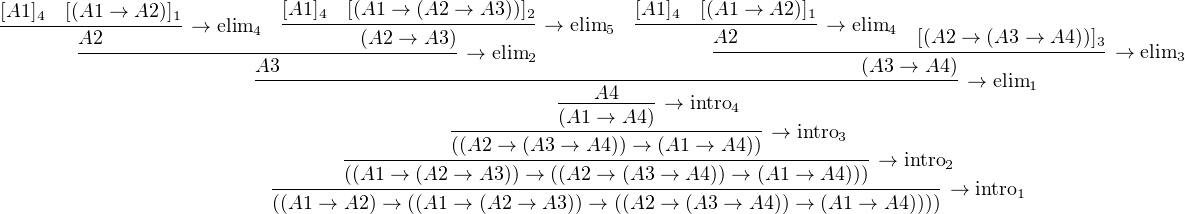
\includegraphics[height=80pt,width=400pt]{images/prooftree0x.png}
    \caption{Prova da fórmula $Fib_{4}$}
    \label{fig:prova_fib_4}
    \end{center}
\end{figure}

\begin{figure}[!ht]
    \begin{center}
        \begin{tikzpicture}[state/.style={rectangle, inner sep=5pt},  node distance=1cm]
            % \tikzstyle{every state}=[circle,thick,minimum size=5mm, text=black,minimum width=1cm]
            \node[state] (C1) {$((A1 \supset A2) \supset ((A1 \supset (A2 \supset A3)) \supset ((A2 \supset (A3 \supset A4)) \supset (A1 \supset A4))))$};
            \node[state] (C2) [above = 0.7cm of C1] {$((A1 \supset (A2 \supset A3)) \supset ((A2 \supset (A3 \supset A4)) \supset (A1 \supset A4)))$};
            \node[state] (C3) [above = 0.7cm of C2] {$((A2 \supset (A3 \supset A4)) \supset (A1 \supset A4))$};
            \node[state] (C4) [above = 0.7cm of C3] {$(A1 \supset A4)$};
            \node[state] (C5) [above = 0.7cm of C4] {$A4$};
            \node[state] (A3) [above left = 0.7cm and 3.2cm of C5] {$A3$};
            \node[state] (A3A4) [above right = 0.7cm and 3.2cm of C5] {$(A3 \supset A4)$};
            \node[state] (A2) [above left = 0.7cm and 1cm of A3] {$A2$};
            \node[state] (A2A3) [above right = 0.7cm and 1cm of A3] {$(A2 \supset A3)$};
            \node[state] (A1_1) [above left = 0.7cm and -0.3cm of A2] {$A1$};
            \node[state] (A1A2_1) [above right = 0.7cm and -0.3cm of A2] {$(A1 \supset A2)$};
            \node[state] (A1_2) [above left = 0.7cm and -0.8cm of A2A3] {$A1$};
            \node[state] (A1A2A3) [above right = 0.7cm and -1.2cm of A2A3] {$A1 \supset (A2 \supset A3)$};
            \node[state] (A2_2) [above left = 0.7cm and 0.5cm of A3A4] {$A2$};
            \node[state] (A2A3A4) [above right = 0.7cm and -2.5cm of A3A4] {$A2 \supset (A3 \supset A4)$};
            \node[state] (A1_3) [above left = 0.7cm and -0.3cm of A2_2] {$A1$};
            \node[state] (A1A2_2) [above right = 0.7cm and -0.3cm of A2_2] {$(A1 \supset A2)$};
            
            \path[-latex]  (C2) edge [thick, left] (C1);
            \path[-latex]  (C3) edge [thick, left] (C2);
            \path[-latex]  (C4) edge [thick, left] (C3);
            \path[-latex]  (C5) edge [thick, left] (C4);
            \path[-latex]  (A3) edge [thick, left] (C5);
            \path[-latex]  (A3A4) edge [thick, left] (C5);
            \path[-latex]  (A2) edge [thick, left] (A3);
            \path[-latex]  (A2A3) edge [thick, left] (A3);
            \path[-latex]  (A1_1) edge [thick, left] (A2);
            \path[-latex]  (A1A2_1) edge [thick, left] (A2);
            \path[-latex]  (A1_2) edge [thick, left] (A2A3);
            \path[-latex]  (A1A2A3) edge [thick, left] (A2A3);
            \path[-latex]  (A2_2) edge [thick, left] (A3A4);
            \path[-latex]  (A2A3A4) edge [thick, left] (A3A4);
            \path[-latex]  (A1_3) edge [thick, left] (A2_2);
            \path[-latex]  (A1A2_2) edge [thick, left] (A2_2);
            
            % \path[-latex]  (a1_2) edge [thick, left] node {0} (a2_2);
            % \path[-latex]  (a1a2_2) edge [thick, right] node {0} (a2_2);
            % \path[-latex]  (a2_2) edge [thick, left] node {0} (a3a4);
            % \path[-latex]  (a3a4) edge [thick, left, dotted] (sa3a4);
        \end{tikzpicture}
        \caption{EGDD da derivação de $Fib_4$}
        \label{fig:der_fib4}
    \end{center}
\end{figure}

Neste Capítulo utilizamos como métrica para o tamanho de uma prova o tamanho do grafo direcionado que o representa (\textit{quantidade de vértices} $+$ \textit{quantidade de arestas}).

O grafo que representa a prova de $Fib_4$ possui tamanho 40 (17 \textit{vértices} $+$ 16 \textit{arestas dedutivas} $+$ 7 \textit{arestas de descarte}), antes de iniciar a compressão, as arestas de descarte são substituídas pelas cadeias de bits de dependências associadas a cada aresta dedutiva, logo, o tamanho do grafo antes de inciar a compressão é 33.

% Na dedutiva, o t. A representação em DOT da prova possui xxx caracteres.aresta compressão da prova de $Fib_4$ são executados 4 colapsos de vértices. Considerando o nível da conclusão como o nível 1, até o nível 6 nenhum colapso é realizado; no nível 7, existem 2 vértices rotulados com 'A2' resultando em 1 colapso; no nível 8, existem 3 vértices rotulados com 'A2' resultando em 2 colapsos e existem 2 vértices rotulados com '$A1 \supset A2$' resultando em 1 colapso.

Considerando o nível da conclusão como o nível 1, o primeiro colapso é realizado no nível 7 entre os 2 vértices rotulados com a fórmula 'A2'.

\begin{center}
    \begin{tikzpicture}[state/.style={rectangle, inner sep=5pt},  node distance=1cm]
        % \tikzstyle{every state}=[circle,thick,minimum size=5mm, text=black,minimum width=1cm]
        \node[state] (a3) {$A3$};
        \node[circle,fill,inner sep=1.5pt] (sa3) [below = 1cm of a3] {};
        \node[state] (a2_1) [above = 1cm of a3] {$\boldsymbol{A2}$};
        \node[state] (a1_1) [above left = 1.25cm and 0cm of a2_1] {$A1$};
        \node[state] (a1a2_1) [above right = 1.25cm and 0cm of a2_1] {$A1 \mysupset A2$};
        
        \node[state] (a3a4) [right = 4cm of a3] {$A3 \supset A4$};
        \node[circle,fill,inner sep=1.5pt] (sa3a4) [below = 1cm of a3a4] {};
        \node[state] (a2_2) [above = 1cm of a3a4] {$\boldsymbol{A2}$};
        \node[state] (a1_2) [above left = 1.25cm and 0cm of a2_2] {$A1$};
        \node[state] (a1a2_2) [above right = 1.25cm and 0cm of a2_2] {$A1 \mysupset A2$};
        
        \path[-latex]  (a1_1) edge [thick, left] node {0} (a2_1);
        \path[-latex]  (a1a2_1) edge [thick, right] node {0} (a2_1);
        \path[-latex]  (a2_1) edge [thick, left] node {0} (a3);
        \path[-latex]  (a3) edge [thick, left, dotted] (sa3);
        
        \path[-latex]  (a1_2) edge [thick, left] node {0} (a2_2);
        \path[-latex]  (a1a2_2) edge [thick, right] node {0} (a2_2);
        \path[-latex]  (a2_2) edge [thick, left] node {0} (a3a4);
        \path[-latex]  (a3a4) edge [thick, left, dotted] (sa3a4);
    \end{tikzpicture}
\end{center}

\noindent Como ambos os vértices possuem 2 premissas e ainda não foram colapsados, são adicionadas 4 arestas de ancestralidade.

\begin{center}
    \begin{tikzpicture}[state/.style={rectangle, inner sep=5pt},  node distance=1cm]
        % \tikzstyle{every state}=[circle,thick,minimum size=5mm, text=black,minimum width=1cm]
        \node[state] (a2) {$\boldsymbol{A2}$};
        
        \node[state] (a3) [below left = 1.25cm and 0cm of a2] {$A3$};
        \node[state] (a3a4) [below right = 1.25cm and 0cm of a2] {$A3 \supset A4$};
        \node[circle,fill,inner sep=1.5pt] (sa3) [below = 1cm of a3] {};
        \node[circle,fill,inner sep=1.5pt] (sa3a4) [below = 1cm of a3a4] {};
        
        \node[state] (a1_1) [above left = 1.25cm and 2cm of a2] {$A1$};
        \node[state] (a1a2_1) [above left = 1.25cm and 0.1cm of a2] {$A1 \mysupset A2$};
        \node[state] (a1_2) [above right = 1.25cm and 0.1cm of a2] {$A1$};
        \node[state] (a1a2_2) [above right = 1.25cm and 2cm of a2] {$A1 \mysupset A2$};
        
        \path[-latex]  (a1_1) edge [thick, left] node {0} (a2);
        \path[-latex]  (a1a2_1) edge [thick, right] node {0} (a2);
        \path[-latex]  (a2) edge [thick, left] node {1} (a3);
        \path[-latex]  (a3) edge [thick, left, dotted] (sa3);
        
        \path[-latex]  (a1_2) edge [thick, left] node {0} (a2);
        \path[-latex]  (a1a2_2) edge [thick, right] node {0} (a2);
        \path[-latex]  (a2) edge [thick, right] node {2} (a3a4);
        \path[-latex]  (a3a4) edge [thick, left, dotted] (sa3a4);
        
        \path[-latex] (a3) edge [thick, left, dashed, bend left=20] node {0;1} (a1_1);
        \path[-latex] (a3) edge [thick, left, dashed, bend left=10] node {0;1} (a1a2_1);
        
        \path[-latex] (a3a4) edge [thick, right, dashed, bend right=10] node {0;2} (a1_2);
        \path[-latex] (a3a4) edge [thick, right, dashed, bend right=20] node {0;2} (a1a2_2);
    \end{tikzpicture}
\end{center}
 
No nível 8, o primeiro de dois colapsos dos vértices rotulados com 'A1' é realizado com os dois vértices que possuem uma aresta dedutiva apontando para o vértice rotulado com 'A2', colapsado no nível inferior. Ambos os vértices são premissas e cada um possui uma aresta de ancestralidade incidente.

\begin{center}
    \begin{tikzpicture}[state/.style={rectangle, inner sep=5pt},  node distance=1cm]
        % \tikzstyle{every state}=[circle,thick,minimum size=5mm, text=black,minimum width=1cm]
        \node[state] (a2) {$A2$};
        \node[state] (a1_1) [above left =  1.25cm and 0cm of a2] {$\boldsymbol{A1}$};
        \node[state] (a1_2) [above right =  1.25cm and 0cm of a2] {$\boldsymbol{A1}$};
        \node[state] (a3) [below left =  1.25cm and 0cm of a2] {$A3$};
        \node[state] (a3a4) [below right =  1.25cm and 0cm of a2] {$A3 \supset A4$};
        
        \node[circle,fill,inner sep=1.5pt] (sa3) [below = 1cm of a3] {};
        \node[circle,fill,inner sep=1.5pt] (sa3a4) [below = 1cm of a3a4] {};
        
        \path[-latex]  (a1_1) edge [thick, left] node {0} (a2);
        \path[-latex]  (a1_2) edge [thick, right] node {0} (a2);
        \path[-latex]  (a3) edge [thick, left, dotted] (sa3);
        \path[-latex]  (a3a4) edge [thick, left, dotted] (sa3a4);
        \path[-latex]  (a2) edge [thick, left] node {1} (a3);
        \path[-latex]  (a2) edge [thick, right] node {2} (a3a4);
        \path[-latex]  (a3) edge [thick, left, dashed, bend left = 20] node {0;1} (a1_1);
        \path[-latex]  (a3a4) edge [thick, right, dashed, bend right = 20] node {0;2} (a1_2);
    \end{tikzpicture}
\end{center}

\noindent Além do colapso dos vértices, as arestas dedutivas que possuem o vértice 'V2' como destino também são colapsadas. A aresta colapsada é rotulada com a cor especial $\lambda$ e com as cores das arestas dedutivas colapsadas, que nesse caso é somente a cor 0. Como os vértices não possuem premissas, as arestas de ancestralidade incidentes são rebaixadas e seus respectivos rótulos são atualizados.

\begin{center}
    \begin{tikzpicture}[state/.style={rectangle, inner sep=5pt},  node distance=1cm]
        % \tikzstyle{every state}=[circle,thick,minimum size=5mm, text=black,minimum width=1cm]
        \node[state] (a2) {$A2$};
        \node[state] (a1_1) [above =  1cm of a2] {$\boldsymbol{A1}$};
        \node[state] (a3) [below left =  1.25cm and 0cm of a2] {$A3$};
        \node[state] (a3a4) [below right =  1.25cm and 0cm of a2] {$A3 \supset A4$};
        
        \node[circle,fill,inner sep=1.5pt] (sa3) [below = 1cm of a3] {};
        \node[circle,fill,inner sep=1.5pt] (sa3a4) [below = 1cm of a3a4] {};
        
        \path[-latex]  (a1_1) edge [thick, left] node {$\lambda_{\{0\}}$} (a2);
        \path[-latex]  (a3) edge [thick, left, dotted] (sa3);
        \path[-latex]  (a3a4) edge [thick, left, dotted] (sa3a4);
        \path[-latex]  (a2) edge [thick, left] node {1} (a3);
        \path[-latex]  (a2) edge [thick, right] node {2} (a3a4);
        \path[-latex]  (a3) edge [thick, left, dashed, bend left = 40] node {1} (a2);
        \path[-latex]  (a3a4) edge [thick, right, dashed, bend right = 40] node {2} (a2);
    \end{tikzpicture}
\end{center}

O vértice resultante do colapso anterior é colapsado com o outro vértice rotulado com 'A1' no nível 8 e que também não possui premissas. O vértice 'A2' possui 2 arestas de ancestralidade incidentes, mas elas não interferem no colapso. 

\begin{center}
    \begin{tikzpicture}[state/.style={rectangle, inner sep=5pt},  node distance=1cm]
        % \tikzstyle{every state}=[circle,thick,minimum size=5mm, text=black,minimum width=1cm]
        \node[state] (a1_1) {$\boldsymbol{A1}$};
        \node[state] (a2) [below =  1cm of a1_1] {$A2$};
        \node[circle,fill,inner sep=1.5pt] (sa2) [below = 1cm of a2] {};
        
        \node[state] (a1_2) [right =  4cm of a1_1] {$\boldsymbol{A1}$};
        \node[state] (a2a3) [below =  1cm of a1_2] {$A2 \supset A3$};
        \node[circle,fill,inner sep=1.5pt] (sa2a3) [below = 1cm of a2a3] {};
        
        \path[-latex]  (a1_1) edge [thick, left] node {$\lambda_{\{0\}}$} (a2);
        \path[-latex]  (a2) edge [thick, left, dotted] (sa2);
        
        \path[-latex]  (a1_2) edge [thick, left] node {0} (a2a3);
        \path[-latex]  (a2a3) edge [thick, left, dotted] (sa2a3);
    \end{tikzpicture}
\end{center}

\noindent Após o colapso, apenas um vértice é removido do grafo.

\begin{center}
    \begin{tikzpicture}[state/.style={rectangle, inner sep=5pt},  node distance=1cm]
        % \tikzstyle{every state}=[circle,thick,minimum size=5mm, text=black,minimum width=1cm]
        \node[state] (a1_1) {$\boldsymbol{A1}$};
        \node[state] (a2) [below left =  1.25cm and 0cm of a1_1] {$A2$};
        \node[circle,fill,inner sep=1.5pt] (sa2) [below = 1cm of a2] {};
        
        \node[state] (a2a3) [below right =  1.25cm and 0cm of a1_1] {$A2 \supset A3$};
        \node[circle,fill,inner sep=1.5pt] (sa2a3) [below = 1cm of a2a3] {};
        
        \path[-latex]  (a1_1) edge [thick, left] node {$\lambda_{\{0\}}$} (a2);
        \path[-latex]  (a2) edge [thick, left, dotted] (sa2);
        
        \path[-latex]  (a1_1) edge [thick, right] node {0} (a2a3);
        \path[-latex]  (a2a3) edge [thick, left, dotted] (sa2a3);
    \end{tikzpicture}
\end{center}

O último colapso, ainda no nível 8, envolve os dois vértices rotulados com $A1 \supset A2$. Ambos os vértices não possuem premissas e cada um possui uma aresta de ancestralidade incidente.

\begin{center}
    \begin{tikzpicture}[state/.style={rectangle, inner sep=5pt},  node distance=1cm]
        % \tikzstyle{every state}=[circle,thick,minimum size=5mm, text=black,minimum width=1cm]
        \node[state] (a2) {$A2$};
        \node[state] (a1_1) [above left =  1.25cm and 0cm of a2] {$\boldsymbol{A1 \supset A2}$};
        \node[state] (a1_2) [above right =  1.25cm and 0cm of a2] {$\boldsymbol{A1 \supset A2}$};
        \node[state] (a3) [below left =  1.25cm and 0cm of a2] {$A3$};
        \node[state] (a3a4) [below right =  1.25cm and 0cm of a2] {$A3 \supset A4$};
        
        \node[circle,fill,inner sep=1.5pt] (sa3) [below = 1cm of a3] {};
        \node[circle,fill,inner sep=1.5pt] (sa3a4) [below = 1cm of a3a4] {};
        
        \path[-latex]  (a1_1) edge [thick, left] node {0} (a2);
        \path[-latex]  (a1_2) edge [thick, right] node {0} (a2);
        \path[-latex]  (a3) edge [thick, left, dotted] (sa3);
        \path[-latex]  (a3a4) edge [thick, left, dotted] (sa3a4);
        \path[-latex]  (a2) edge [thick, left] node {1} (a3);
        \path[-latex]  (a2) edge [thick, right] node {2} (a3a4);
        \path[-latex]  (a3) edge [thick, left, dashed, bend left = 20] node {0;1} (a1_1);
        \path[-latex]  (a3a4) edge [thick, right, dashed, bend right = 20] node {0;2} (a1_2);
    \end{tikzpicture}
\end{center}

\noindent Esse colapso é semelhante ao primeiro colapso dos vértices $A1$, no entanto, as arestas de ancestralidade são removidas em vez de serem rebaixadas, pois, já existem arestas de ancestralidade de A3 para A2, e de $A3 \supset A4$ para A2 com os mesmos rótulos. Esse colapso remove 3 arestas, sendo 1 dedutiva e 2 de ancestralidade.

\begin{center}
     \begin{tikzpicture}[state/.style={rectangle, inner sep=5pt},  node distance=1cm]
        % \tikzstyle{every state}=[circle,thick,minimum size=5mm, text=black,minimum width=1cm]
        \node[state] (a2) {$A2$};
        \node[state] (a1_1) [above =  1cm of a2] {$\boldsymbol{A1 \supset A2}$};
        \node[state] (a3) [below left =  1.25cm and 0cm of a2] {$A3$};
        \node[state] (a3a4) [below right =  1.25cm and 0cm of a2] {$A3 \supset A4$};
        
        \node[circle,fill,inner sep=1.5pt] (sa3) [below = 1cm of a3] {};
        \node[circle,fill,inner sep=1.5pt] (sa3a4) [below = 1cm of a3a4] {};
        
        \path[-latex]  (a1_1) edge [thick, left] node {$\lambda_{\{0\}}$} (a2);
        \path[-latex]  (a3) edge [thick, left, dotted] (sa3);
        \path[-latex]  (a3a4) edge [thick, left, dotted] (sa3a4);
        \path[-latex]  (a2) edge [thick, left] node {1} (a3);
        \path[-latex]  (a2) edge [thick, right] node {2} (a3a4);
    \end{tikzpicture}
\end{center}

A Tabela \ref{tab:col_tam} mostra o tamanho do grafo em cada colapso. Apesar de não ser a métrica que descreve o real de tamanho da prova, pois são adicionadas informações às arestas durante a compressão, o tamanho do grafo evidencia o comportamento da Compressão Horizontal durante a compressão de uma prova. Nos primeiros colapsos o tamanho do grafo de prova é superior ao tamanho do grafo antes da compressão, mas a medida que colapsos vão sendo executados e vértices e arestas são retirados, o tamanho do grafo tende a diminuir. 

\begin{table} [!ht]
    \caption{Tamanho do grafo direcionado em cada colapso}\label{tab:col_tam}
    ~\\[-2mm]
    \begin{tabularx}{\textwidth}{@{\extracolsep{0pt}}C @{\extracolsep{0pt}}C C}

        \textbf{Passo}
        & \textbf{Tamanho (vértices + arestas)}
        \\\toprule

        ~ \\[-6mm]
        grafo inicial
        & 33 (17 + 16)
        \\\midrule
    
        ~ \\[-6mm]
        colapso 1
        & 36 (16 + 20)
        \\\midrule
    
        ~ \\[-6mm]
        colapso 2
        & 34 (15 + 19)
        \\\midrule
    
        ~ \\[-6mm]
        colapso 3
        & 33 (14 + 19)
        \\\midrule
        
        ~ \\[-6mm]
        colapso 4
        & 29 (13 + 16)
        \\\midrule
    \end{tabularx}
\end{table}

O Capítulo \ref{cap:impl_exp} apresenta como os grafos de prova (EGDD) da Compressão Horizontal são representados em arquivos e o Capítulo \ref{cap:experimentos} apresenta os resultados de compressão utilizando a representação em arquivos de texto.
  % -*- coding: utf-8; -*-

\chapter{Implementação da Compressão Horizontal}
\label{cap:impl_exp}

Esse capítulo apresenta a implementação do \textit{compressing}\footnote{\href{https://github.com/flavio-barros/compressing}{https://github.com/flavio-barros/compressing}}, compressor de provas que executa o algoritmo da Compressão Horizontal apresentado por Gordeev e Haeusler \cite{GordeevH16}. O objetivo desta implementação é fornecer os primeiros resultados empíricos da compressão e auxiliar na definição do algoritmo, aperfeiçoando procedimentos e estruturas de dados utilizadas durante o processo de compressão.

\section{Decisões de Projeto}

A finalização da formalização do algoritmo da Compressão Horizontal foi realizada paralelamente à implementação do \textit{compressing}, essa implementação tinha o objetivo inicial de retroalimentar a formalização do algoritmo com informações sobre a sua execução. Para gerar as informações sobre a execução do algoritmo seria necessário documentar os passos de execução através da geração de visualizações do grafo de prova durante o processo de compressão. Além da geração das visualizações, outro fator importante considerado durante a definição das decisões de projeto foi a necessidade de realizar várias modificações no código do compressor durante o desenvolvimento.

O \textit{compressing} foi implementado utilizando a linguagem de programação \textit{Python}. A escolha da linguagem levou em consideração a existência de uma implementação inicial da Compressão Horizontal escrita em Python, além de que a linguagem não demanda muito esforço para alterações no código e ainda possui várias bibliotecas com suporte a operações em grafos que possuem integração com o pacote de ferramentas de visualizações de grafos \textit{graphviz}.

\section{Estrutura do Projeto}

Utilizamos o padrão de projeto \textit{Adapter} para estruturar o projeto. A adoção do Adapter na estruturação do sistema permite a integração de classes externas ao sistema, convertendo a interface das classes externas à uma interface esperada pelas classes internas. 

A Figura \ref{fig:diag_adapter} mostra um exemplo de como as classes são estruturadas utilizando o \textit{Adapter}. Na \textit{Interface} são definidos os métodos que uma classe interna espera. A classe \textit{Adaptador} implementa a interface e utiliza os métodos da classe externa (\textit{ClasseAdaptada}) para definir os métodos esperados pela classe interna (\textit{ClasseCliente}).

\begin{figure}[ht]
  \begin{center}
    \fbox{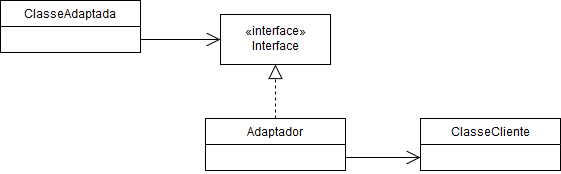
\includegraphics[height=80pt,width=257pt]{images/DiagramaClasse.png}}
    \caption{Exemplo de diagrama de classes do \textit{Adapter}}
    \label{fig:diag_adapter}
  \end{center}
\end{figure}

No \textit{compressing}, as classes adaptadas são dos pacotes que fornecem as funcionalidades de manipulação e visualização de grafos. A Figura \ref{fig:diag_comp} mostra o diagrama de classes simplificado do \textit{compressing}. A classe \textit{GraphAdapter} possui um objeto da classe \textit{DiGraph} e implementa a interface \textit{Graph}, que define todos os métodos de manipulação de grafos utilizados no \textit{compressing}. A implementação de cada método da classe \textit{GraphAdapter} adapta as funcionalidades oferecidas pela \textit{DiGraph}, que pertence ao pacote \textit{networkx}\footnote{\href{https://networkx.github.io/}{https://networkx.github.io/}}, para as funcionalidades definidas pela interface \textit{Graph}. A classe \textit{ProofGraph} implementa a EGDD definida na Seção \ref{sec:comp_hor} utilizando um objeto da classe \textit{GraphAdapter}. De maneira semelhante, a classe \textit{VisualGraphAdapter} converte as funcionalidades da classe \textit{Agraph}, do pacote pygraphviz\footnote{\href{https://pygraphviz.github.io/}{https://pygraphviz.github.io/}}, implementando os métodos definidos pela interface \textit{VisualGraph}. A principal diferença é que a \textit{VisualGraphAdapter} é utilizada por duas classes: a classe \textit{VisualProofGraph} implementa a visualização do do grafo de um objeto da \textit{ProofGraph}; a classe \textit{VisualCollapseGraph} implementa a geração da visualização de um colapso do processo de compressão, que é um subgrafo do grafo de um objeto da \textit{ProofGraph}.

\begin{figure}[ht]
  \begin{center}
    \fbox{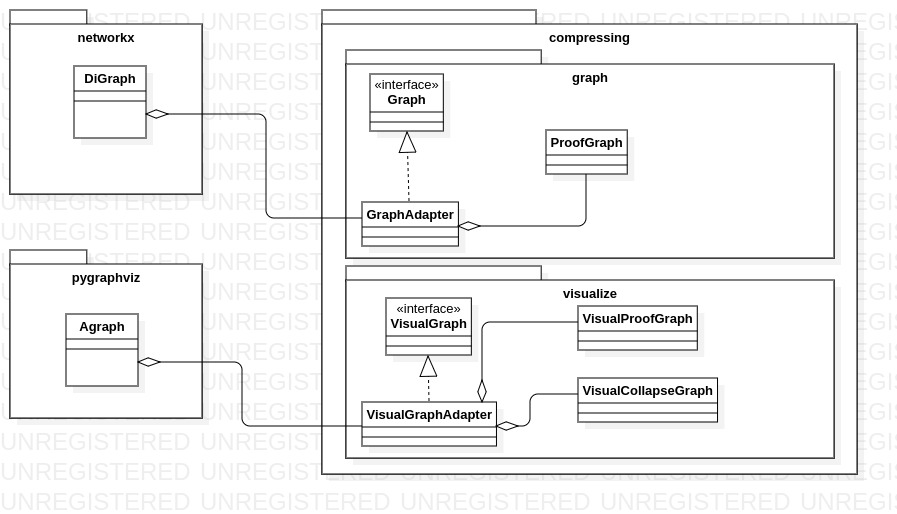
\includegraphics[height=230pt,width=400pt]{images/diagrama_classes.jpg}}
    \caption{Diagrama de classes simplificado do \textit{compressing}}
    \label{fig:diag_comp}
  \end{center}
\end{figure}

\section{Representação das Provas}

Os grafos de prova são representados por arquivos DOT, linguagem de descrição de grafos do \textit{graphviz}. A linguagem DOT pode representar grafos direcionados e não direcionados; subgrafos; atributos de grafos, vértices e arestas. O \textit{compressing} aceita somente arquivos \textit{.dot} que seguem as seguintes convenções:

\begin{itemize}
    \item Cada vértice do grafo é identificado por um \textit{id} e possui um atributo \textit{label}, que tem como valor a fórmula a qual o vértice é associado.
    \item Cada aresta de descarte possui um atributo \textit{comment} com o valor \textit{discharge}.
    \item As arestas dedutivas não possuem qualquer informação adicional.
\end{itemize}

Cada arquivo de saída possui as informações da EGDD adicionadas durante a compressão na forma de atributos de grafo, vértices e arestas. Cada arquivo gerado pelo \textit{compressing} segue as seguintes convenções:

\begin{itemize}
    \item A representação dos vértices é idêntica à dos arquivos de entrada.
    \item As arestas dedutivas que \textbf{não foram} colapsadas durante a compressão possuem três atributos: \textit{collapsed}, que possui valor \textit{False} indicando que a aresta não foi colapsada; \textit{color}, que possui como valor o numeral que indica sua cor; \textit{dependencies}, que possui como valor a cadeia de bits que indicam a dependência da fórmula do vértice que é sua origem.
    \item As arestas dedutivas que \textbf{foram} colapsadas durante a compressão possuem dois atributos: \textit{collapsed}, que possui valor \textit{True} indicando que a aresta foi colapsada; \textit{lambda-colors}, que possui como valor as cores das arestas dedutivas que a originaram.
    \item As arestas de ancestralidade possuem apenas um atributo, \textit{path}, que possui uma lista de cores que representa o caminho, através de arestas dedutivas, entre o vértice que é seu destino e o vértice que é a sua origem.
    \item O grafo possui um atributo, \textit{order}, que possui como valor a lista de fórmulas representando a ordenação linear utilizada para a construção das cadeias de bits de dependências.
\end{itemize}


  % -*- coding: utf-8; -*-

\chapter{Experimentos}
\label{cap:experimentos}

Este capítulo apresenta os resultados dos experimentos das técnicas de compressão aplicadas a um conjunto de provas de tautologias da M$\supset$.

\section{Ambiente Computacional}

Todos os experimentos relatados nesta Seção foram executados em uma máquina com processador Intel Core i3-6100U 2,30GHz, 8GB de memória RAM e com sistema operacional Ubuntu 18.04.1 LTS. O \textit{gerador de fórmulas}\footnote{\label{ftn:impl_ger_huff}\href{https://github.com/flavio-barros/proof-compressions}{https://github.com/flavio-barros/proof-compressions}} descrito na Seção \ref{sec:base_dados} e a \textit{implementação da codificação de Huffman}\footref{ftn:impl_ger_huff}, cujos resultados de compressão são mostrados na Seção \ref{sec:resultados}, foram implementados utilizando a linguagem \textit{Python}.

\section{Provas de Entrada}
\label{sec:base_dados}

Provas com tamanho super-polinomial em relação ao tamanho da conclusão são redundantes, quanto maior a prova, maior a quantidade de redundâncias \cite{GorHae2019}. Em um árvore de prova, essas redundâncias são ramos idênticos que se repetem ao longo da prova no mesmo nível da derivação. Portanto, para a Compressão Horizontal, quanto maior a prova, maior a quantidade de colapsos e consequentemente, maior a taxa de compressão. Como observado no Capítulo \ref{cap:aplicacao_tec}, quando aplicada a provas que permitem poucos colapsos, a CH gera provas maiores que as originais. Logo, o conjunto de provas utilizadas nos experimentos deve ser necessariamente composto por provas grandes, que possuem tamanhos exponenciais em relação ao tamanho da conclusão, para que seja possível mensurar a capacidade de compressão da CH.

Inicialmente, consideramos três famílias de fórmulas para serem utilizadas nos experimentos. A primeira família de fórmulas $\psi_{n}$ definida em \cite{haeusler2015many}, não possui provas normais, para qualquer $n > 0$, com menos de $2^n$ hipóteses descartadas. $\psi_{n}$ é definida com segue:

\begin{definition}{\textbf{Fórmulas Haeusler.}}
Seja $\chi[X, Y] = (((X \supset Y) \supset X) \supset X) \supset Y$. Considere os símbolos proposicionais $C$ e $D_i$, para $i > 0$. A família de fórmulas $\xi_{i}$ é definida recursivamente como segue:
\begin{align*}
\xi_1 &= \chi[D_1, C] \\
\xi_{i+1} &= \chi[D_{i+1}, \xi_i]
\end{align*}
Utilizando $\xi_i$, a família de fórmulas $\psi_n$, para $n > 0$, é definida como segue, para $i \geq 1$: $$\psi_{i+1} = \xi_{i+1} \supset C$$
\end{definition}

A segunda família de fórmulas foi retirada da Biblioteca ILTP\footnote{\href{http://www.iltp.de/}{http://www.iltp.de/}} (\textit{Intuitionistic Logic Theorem Proving (ILTP) Library}) que fornece uma plataforma para testes para provadores de teoremas da lógica proposicional e de primeira ordem intuicionista. Os problemas da biblioteca estão agrupados em 24 domínios, incluindo o SYJ, domínio dos problemas sintáticos intuicionistas \cite{raths2007iltp}. Um dos problemas, o SYJ204, refere-se a uma família de fórmulas $\phi_n$, tendo apenas a implicação como conectivo, que possui somente provas normais de tamanhos exponenciais. $\phi_n$ é definida como segue:

\begin{definition}{\textbf{Fórmulas SYJ204}.}
Sejam $A_i$, com $i \geq 0$, símbolos proposicionais. A família de fórmulas $\omega_i$ é definida recursivamente como segue:
\begin{align*}
\omega_1 &= (A_1 \supset (A_1 \supset A_0)) \\
\omega_{i+1} &= \omega_i \supset (A_{i+1} \supset (A_{i+1} \supset A_i))
\end{align*}
Utilizando $\omega_i$, a família de fórmulas $\phi_n$, para $n > 0$, é definida como segue, para $i \geq 1$: $$\phi_{i+1} = A_{i+1} \supset (\omega_{i+1} \supset A_0)$$
\end{definition}

A terceira família de fórmulas foi retirada de um exemplo de compressão em \cite{GordeevH16}. $Fib_n$ possui provas normais maiores ou iguais que \textit{fibonacci(n)} e é definida como segue:

\begin{definition}{\textbf{Fórmulas Fibonacci}.}
Sejam $A_i$, com $i \geq 3$, símbolos proposicionais. A família de fórmulas $\sigma_i$ é definida recursivamente como segue:
\begin{align*}
\sigma_3 &= (A_{1} \supset (A_{2} \supset A_{3})) \\
\sigma_{i} &= \sigma_{i-1} \supset (A_{i-2} \supset (A_{i-1} \supset A_{n}))
\end{align*}
Utilizando $\sigma_i$, a família de fórmulas $Fib_n$, para $n > 2$, é definida como segue: $$Fib_{n} = (A_{1} \supset A_2) \supset (\sigma_{n} \supset (A_1 \supset A_n))$$
\end{definition}

As provas utilizadas nos experimentos foram geradas utilizando o provador de teoremas \textit{NatDProver}\footnote{\href{https://github.com/Bpalkmim/NatDProver}{https://github.com/Bpalkmim/NatDProver (Implementação original)}}$^{\text{,}}$\footnote{\href{https://github.com/flavio-barros/NatDProver}{https://github.com/flavio-barros/NatDProver (Implementação alterada para aceitar entradas por linha de comando)}}, desenvolvido no TecMF\footnote{\href{http://www.tecmf.inf.puc-rio.br/}{http://www.tecmf.inf.puc-rio.br/}}, que recebe fórmulas da M$\supset$ e devolve um arquivo \textit{.dot} que contém o grafo de prova caso a prova seja gerada com sucesso. O NatDProver ainda está em desenvolvimento, alguns erros e comportamento inesperados podem ocorrer durante a geração das provas.

Executamos o NatDProver para instâncias das três famílias de fórmulas selecionadas para os experimentos. O provador pode apresentar cinco tipos de retorno em cada execução: \textit{sucesso}, geração da prova e do arquivo \textit{.dot} ocorreram com sucesso; \textit{erro geração DOT}, a geração da prova ocorreu com sucesso, mas a geração do arquivo \textit{.dot} apresentou erro; \textit{erro geração prova}, ocorreu um erro na geração da prova; \textit{falha geração prova}, a geração da prova falhou, mas não ocorreram erros durante a execução; \textit{timeout}, o tempo de execução do provador atingiu o limite de tempo definido.

A Tabela \ref{tab:fam_form_exec} mostra o retorno obtido do NatDProver para cada instância das famílias de fórmulas consideradas. Executamos o provador para 20 instâncias de cada família, o limite de tempo de execução para cada instância foi de 30 minutos.

\begin{table} [!ht]
    \caption{Retornos do NatDProver para cada instâncias das famílias de fórmulas}\label{tab:fam_form_exec}
    ~\\[-2mm]
    \begin{tabularx}{\textwidth}{@{\extracolsep{0pt}}C @{\extracolsep{0pt}} P{2.5cm} C C}

        \hline
        \textbf{Família de fórmulas   } & \textbf{Valor de n} & \textbf{Retorno} \\ \hline
        \multirow{2}{*}{$\psi_n$ (fórmulas Haeusler)} & 1 & \textit{erro geração DOT} \\ \cline{2-3} 
         & 2 - 20 & \textit{falha geração prova} \\ \hline
        \multirow{3}{*}{$\phi_n$ (SYJ204)} & 1 & \textit{sucesso} \\ \cline{2-3} 
         & 2 - 4 & \textit{erro geração DOT} \\ \cline{2-3} 
         & 5 - 20 & \textit{falha geração prova} \\ \hline
        \multirow{2}{*}{$Fib_n$ (fórmulas Fibonacci)} & 3 - 15 & \textit{sucesso} \\ \cline{2-3} 
         & 16 - 22 & \textit{timeout} \\ \hline
    \end{tabularx}
\end{table}

Após as execuções, o NatDProver não gerou nenhum arquivo \textit{.dot} com provas das fórmulas Haeusler, um arquivo para as fórmulas SYJ204 e 13 arquivos para as fórmulas Fibonacci. Como o objetivo do experimento é observar as taxas de compressão das provas obtidas por cada técnica a medida que o tamanho das provas aumenta, utilizamos apenas as fórmulas Fibonacci para gerar os resultados mostrados na próxima seção.

\section{Resultados}
\label{sec:resultados}

Nos gráficos seguintes, as provas das fórmulas de $Fib_n$ são mostradas em termos dos tamanhos das fórmulas no lugar dos valores de $n$, a prova da fórmula de $n = 3$ possui a conclusão com tamanho $13$, $n = 4$ possui tamanho $19$, e assim por diante, até $n = 15$ com a conclusão com tamanho $85$.

A Figura \ref{fig:prova_oco_form} mostra o gráfico que relaciona os tamanhos das fórmulas da família $Fib_n$, considerando a quantidade de símbolos proposicionais, e os tamanhos de suas respectivas provas, considerando o tamanho do grafo de prova. Na Figura \ref{fig:prova_siz_form}, os tamanhos das provas são mostrados considerando os tamanhos (em \textit{kilobytes}) dos arquivos DOT que as representa.

\begin{figure}[ht]
  \begin{center}
    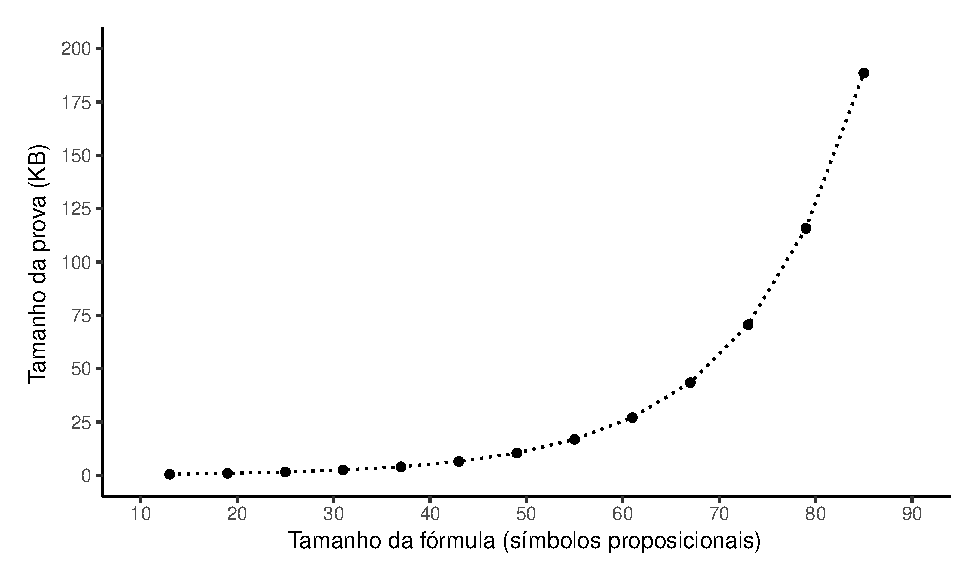
\includegraphics[height=230pt,width=400pt]{images/plot_prova_gra_form.eps}
    \caption{Tamanho das fórmulas e seus respectivos grafos de prova}
    \label{fig:prova_oco_form}
  \end{center}
\end{figure}

\begin{figure}[ht]
  \begin{center}
    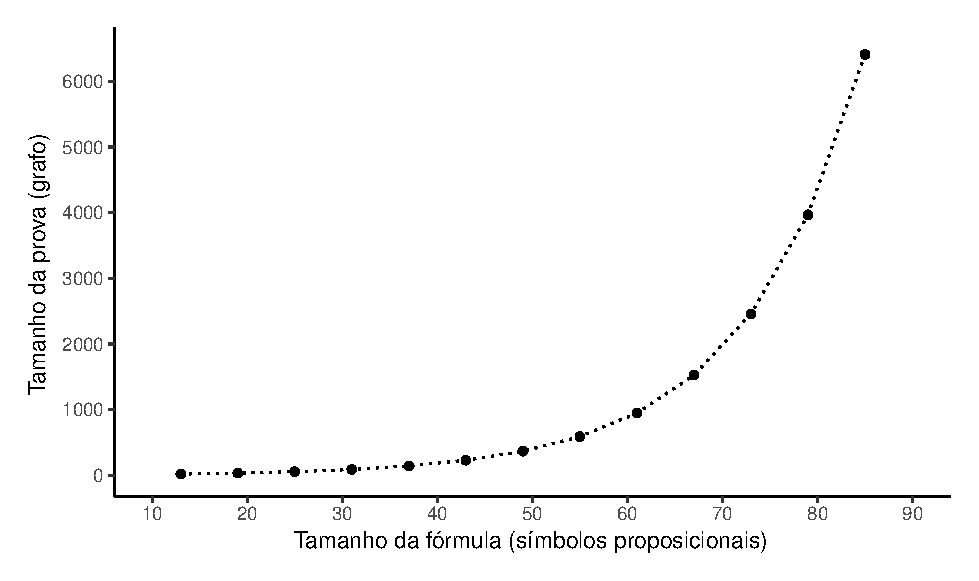
\includegraphics[height=230pt,width=400pt]{images/plot_prova_kb_form.eps}
    \caption{Tamanho das fórmulas e seus respectivos arquivos de prova}
    \label{fig:prova_siz_form}
  \end{center}
\end{figure}

A seguir apresentamos os resultados das aplicações dos algoritmos de compressão às provas das fórmulas de $Fib_n$. Os resultados são mostrados para os algoritmos da codificação de Huffman e da Compressão Horizontal.

A Figura \ref{fig:prova_alg_sizes} mostra os tamanho dos arquivos originais e dos resultantes dos algoritmos de compressão, o eixo dos tamanhos dos arquivos está em escala logarítmica. Como já esperado, a Compressão Horizontal não possui bons resultados para as provas menores, apresentando uma taxa de compressão efetiva apenas a partir da fórmula com tamanho 37 ($n = 7$). A partir da fórmula com tamanho 30 ($n = 8$), a Compressão Horizontal obteve resultados melhores que a codificação de Huffman. A maior prova, da fórmula com tamanho 85 ($n = 15$), possui tamanho original 188,6 KB e foi comprimida para 113 KB pela codificação de Huffman e para 9,36 KB pela Compressão Horizontal.

\begin{figure}[H]
  \begin{center}
    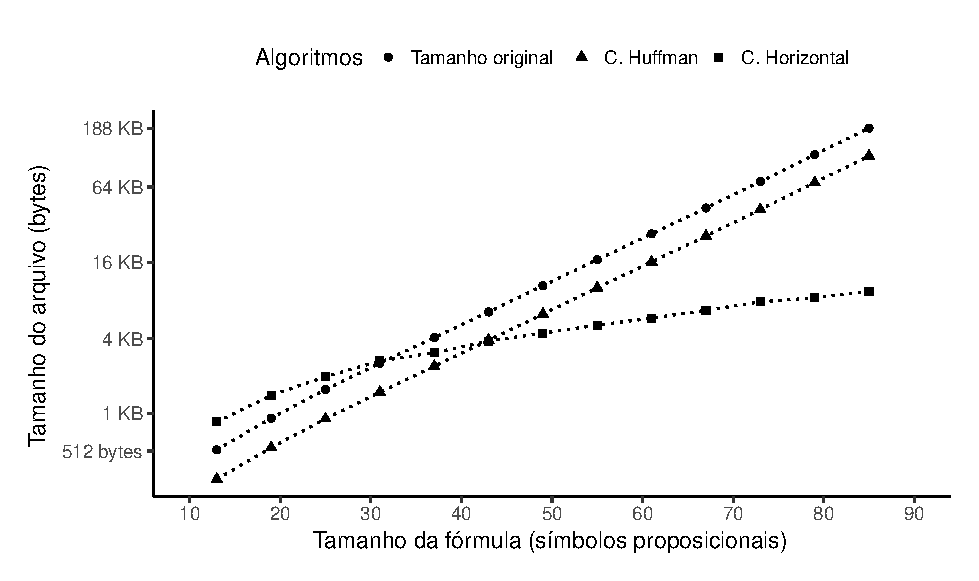
\includegraphics[height=230pt,width=400pt]{images/plot_alg_sizes.eps}
    \caption{Tamanhos dos arquivos de prova após a compressão}
    \label{fig:prova_alg_sizes}
  \end{center}
\end{figure}

A Figura \ref{fig:taxa_comp} mostra as taxas de compressão obtidas para cada fórmula. Para todas as provas, a codificação de Huffman obteve taxa de compressão de aproximadamente 40\%, enquanto que as taxas de compressão da Compressão Horizontal variam bastante de acordo com o tamanho da prova. Para a fórmula de tamanho 13 ($n = 3$), a taxa de compressão obtida foi de -67\% (aumento de 67\% do tamanho do arquivo original) e para a prova da fórmula de tamanho 85 ($n = 15$), a taxa de compressão obtida foi de 95\%.

\begin{figure}[H]
  \begin{center}
    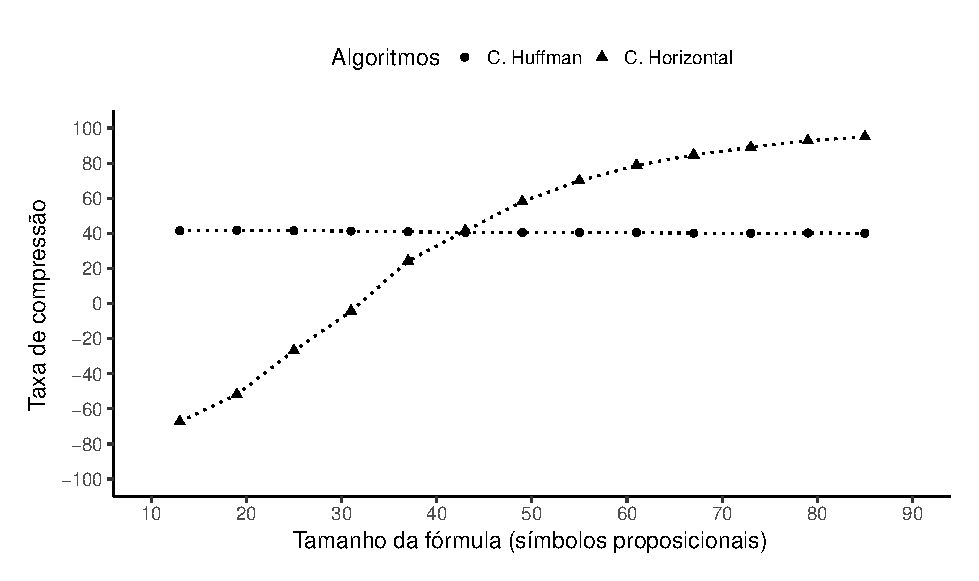
\includegraphics[height=230pt,width=400pt]{images/plot_taxa_comp.eps}
    \caption{Taxa de compressão dos algoritmos}
    \label{fig:taxa_comp}
  \end{center}
\end{figure}

Enquanto que para as taxas de compressão, a Compressão Horizontal obteve resultados mais satisfatórios, para os tempos de execução, a codificação de Huffman apresentou tempos menores para todas as fórmulas. O gráfico da Figura \ref{fig:exec_time} mostra os tempos de execuções dos dois algoritmos para todas as provas, o eixo dos tempos de execução está em escala logarítmica.

\begin{figure}[H]
  \begin{center}
    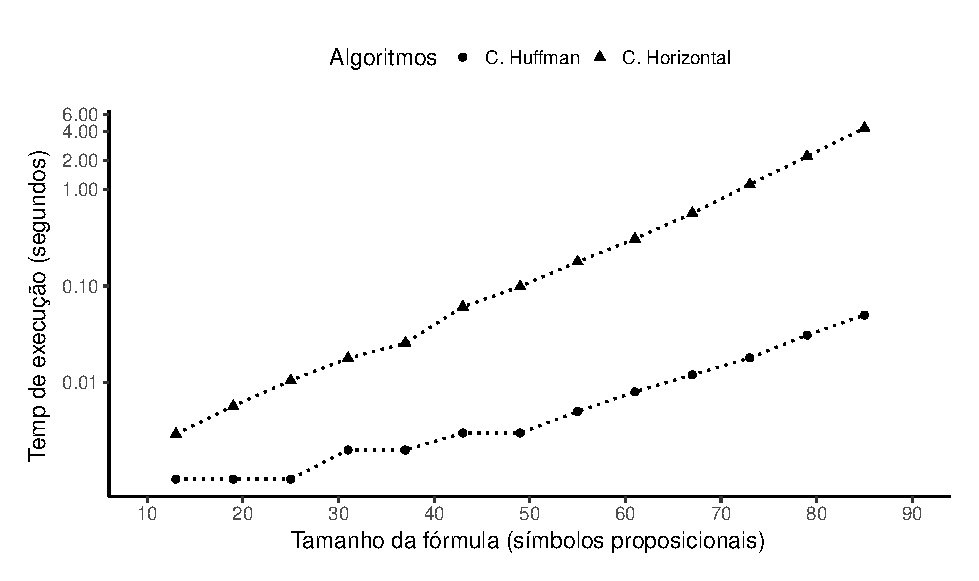
\includegraphics[height=230pt,width=400pt]{images/plot_exec_time.eps}
    \caption{Tempo de execução dos algoritmos de compressão}
    \label{fig:exec_time}
  \end{center}
\end{figure}
  % -*- coding: utf-8; -*-

\chapter{Conclusão e Trabalhos Futuros}
  %% ...
  \arial
  \bibliography{flavio}
  \normalfont

\end{document}
